\documentclass[a4paper, journal]{IEEEtran}
\usepackage[margin=0.75in]{geometry}
\IEEEoverridecommandlockouts
% The preceding line is only needed to identify funding in the first footnote. If that is unneeded, please comment it out.
\usepackage{cite}
\usepackage{amsmath,amssymb,amsfonts}
\usepackage{algorithmic}
\usepackage{graphicx}
\usepackage{textcomp}
\usepackage{listings}
\usepackage{xcolor}
\usepackage{booktabs}
\usepackage{tikz}
\usepackage{times}
\usepackage{newtxmath}


\definecolor{codegreen}{rgb}{0,0.6,0}
\definecolor{codegray}{rgb}{0.5,0.5,0.5}
\definecolor{codepurple}{rgb}{0.58,0,0.82}
\definecolor{backcolour}{rgb}{0.95,0.95,0.92}

\lstset{
  language=Python,
  breaklines=true,
  breakatwhitespace=true,
  basicstyle=\ttfamily\footnotesize,
  keywordstyle=\color{codepurple},
  commentstyle=\color{codegreen},
  stringstyle=\color{red},
  captionpos=b,
  frame=single,
  showstringspaces=false,
  tabsize=4
}


\hyphenation{op-tical net-works semi-conduc-tor IEEE-Xplore}
\def\BibTeX{{\rm B\kern-.05em{\sc i\kern-.025em b}\kern-.08em
    T\kern-.1667em\lower.7ex\hbox{E}\kern-.125emX}}
\usepackage{balance}
\begin{document}

\title{Image Processing Techniques for Image Enhancement and Edge Detection}
\author{
  \IEEEauthorblockN{Bipul Kumar Dahal\IEEEauthorrefmark{1}, Dinanath Padhya\IEEEauthorrefmark{2}, Krishna Acharya\IEEEauthorrefmark{3}} \\
  \IEEEauthorblockA{\IEEEauthorrefmark{1}THA078BEI009 \quad \IEEEauthorrefmark{2}THA078BEI010 \quad \IEEEauthorrefmark{3}THA078BEI020} \quad \\
  Department of Electronics, Communication and Information Engineering\\
  Thapathali Campus, IOE, Tribhuvan University, Nepal\\
}

\maketitle

\begin{abstract}
  This lab report presents the practical steps and results of applying basic image processing techniques to digital photographs. We worked with real images to learn how to read, display, and analyze them using Python libraries. The experiment included separating color channels, plotting histograms, and using filters like Sobel and Laplacian to detect edges. We also added different types of noise to images and then removed them using Gaussian and median filters. The results show how these methods can improve image quality and help in tasks like highlighting important features or cleaning up noisy pictures. These techniques are useful for many applications, including medical imaging, remote sensing, and computer vision.
\end{abstract}
\begin{IEEEkeywords}
  Digital Image Processing, Image Enhancement, Edge Detection, Noise Modeling, Python, OpenCV
\end{IEEEkeywords}

\section{Introduction}
\subsection{Background}

Digital image processing is a crucial field within electronics, communication, and computer engineering, enabling the manipulation and analysis of visual information captured in digital form. With the proliferation of digital cameras, smartphones, and imaging devices, the ability to process and interpret images has become increasingly important for a wide range of applications, including medical imaging, remote sensing, surveillance, robotics, and multimedia. Image processing techniques allow for the enhancement, restoration, segmentation, and analysis of images, making it possible to extract meaningful information, improve visual quality, and automate decision-making processes.

The foundation of image processing lies in understanding how images are represented as matrices of pixel values and how various mathematical and algorithmic operations can be applied to these matrices. Techniques such as filtering, histogram analysis, morphological operations, and edge detection are fundamental tools for enhancing image quality and extracting features. With the advent of powerful open-source libraries like OpenCV, scikit-image, and Matplotlib, implementing and experimenting with these techniques has become accessible to students and researchers, fostering innovation and practical skill development in the field of digital image analysis.

\subsection{Literature Review}
Image enhancement and edge detection have advanced through both classical and modern computational methods. Canny's foundational work (1986) established edge detection principles using Gaussian smoothing, gradient calculation, non-maximum suppression, and hysteresis thresholding \cite{Canny1986}. This mathematically rigorous approach remains a benchmark for its balance between noise robustness and edge localization accuracy. For noise-aware filtering, Tomasi and Manduchi (1998) introduced bilateral filtering, which preserves edges through nonlinear combination of intensity similarities and geometric closeness \cite{Tomasi1998}. This spatial-domain technique inspired numerous variants that maintain structural integrity while reducing noise.

Computational efficiency in feature extraction saw significant improvements through novel convolution designs. Chollet (2017) proposed depthwise separable convolutions in Xception networks, decomposing standard convolutions into spatial and channel-wise operations \cite{Chollet2017}. This factorization reduced computational requirements by 4-10× while maintaining accuracy. Zhang et al. (2017) demonstrated the effectiveness of neural networks for noise reduction with DnCNN, which learns mappings between noisy and clean images using batch normalization and residual connections \cite{Zhang2017}. Their approach showed measurable improvements over non-local means and BM3D on standard benchmarks.

Current methods integrate classical principles with modern computational techniques. Contemporary edge detectors combine Canny's framework with learned representations, while denoising systems incorporate bilateral filtering concepts into attention-based mechanisms. This progression reflects an ongoing development: classical methods provide theoretical foundations and interpretability, while modern computational approaches offer adaptable performance. These combined advances continue to enable progress in medical imaging, autonomous systems, and photographic processing where edge precision and noise handling remain critical challenges.


\subsection{Objectives}
This lab experiment aims to:\
\begin{itemize}
  \item To provide hands-on experience with digital image representation, including reading, displaying, and analyzing images in various formats.
  \item To explore essential image processing techniques such as enhancement, noise modeling, restoration, segmentation, and edge detection using Python libraries.
\end{itemize}


\section{Experiment \& Implementation}
In this section, we present the systematic implementation and analysis of various image processing techniques. Our experiments used three personal photographs as test images, providing a practical context for applying theoretical concepts. We utilized Python libraries including OpenCV, scikit-image, NumPy, and Matplotlib, implementing algorithms for image representation, enhancement, edge detection, segmentation, and noise modeling/restoration.

\subsection{Image Representation}
Digital images are represented as matrices or multi-dimensional arrays of pixel values. In our experiment, we explored both grayscale and color image representations. A color image is typically represented as a 3D array with dimensions representing height, width, and color channels (RGB), while a grayscale image is a 2D array.

Mathematically, an image can be represented as a function $f(x,y)$ where $x$ and $y$ are spatial coordinates, and the amplitude of $f$ at any point $(x,y)$ is the intensity or gray level of the image at that point.

\begin{figure}[htbp]
  \centering
  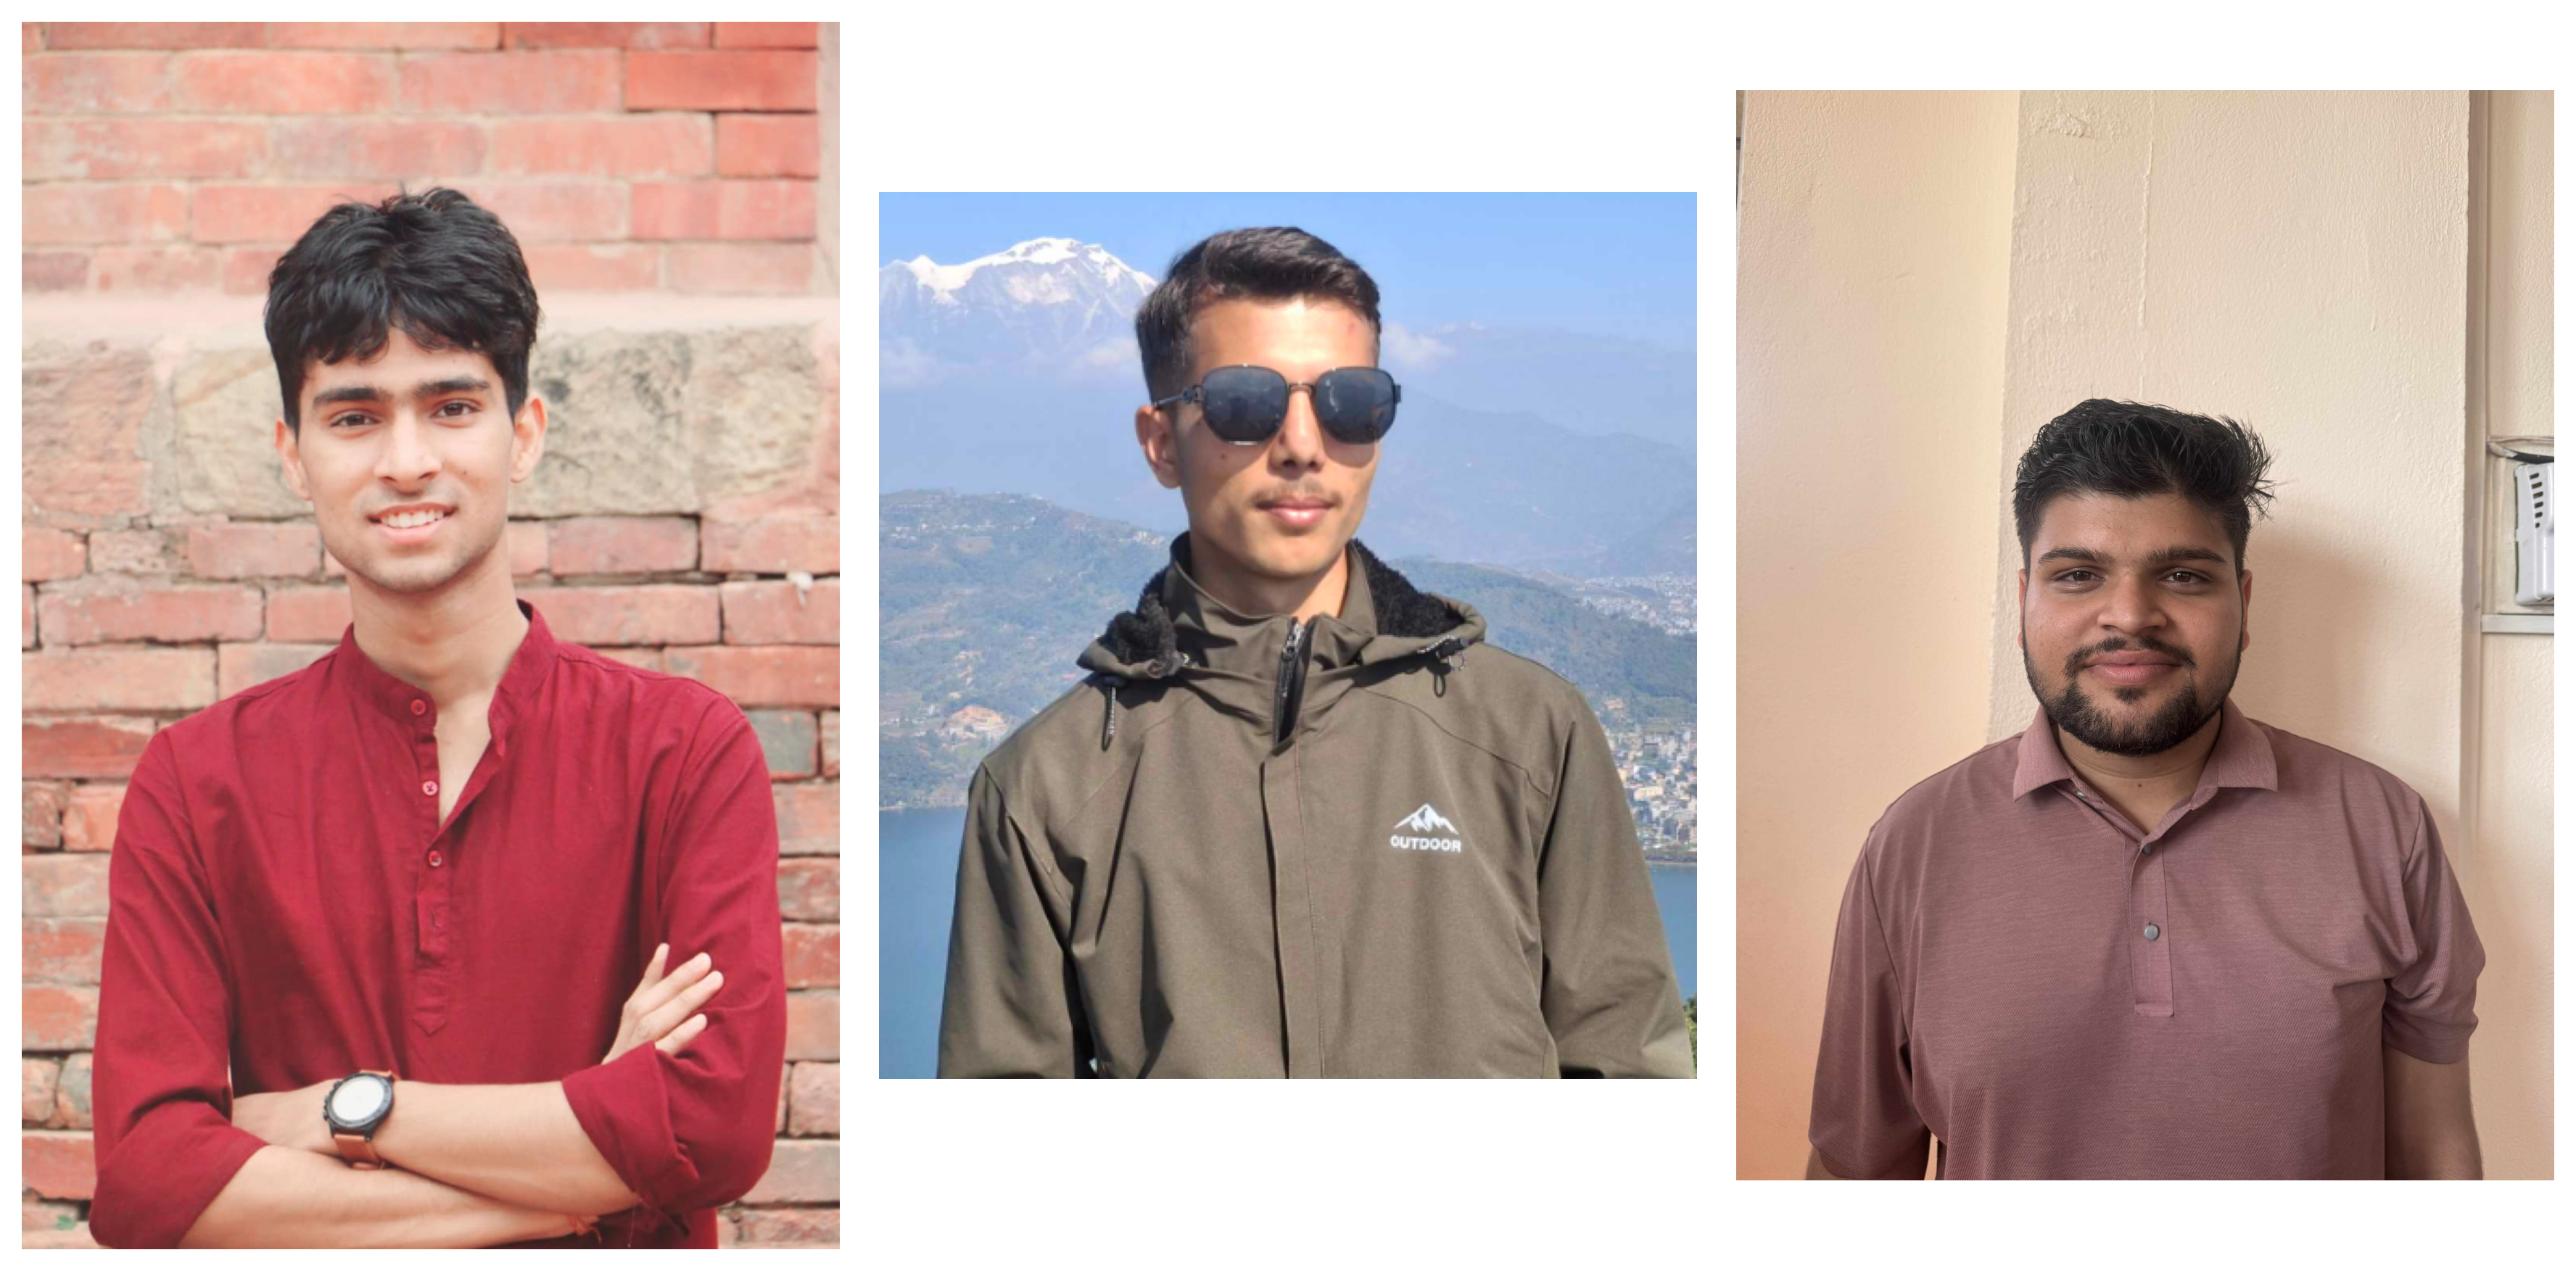
\includegraphics[width=\linewidth]{images/lab1/three_images_rgb.png}
  \caption{RGB representation of the test images}
  \label{fig:test_images}
\end{figure}

\begin{figure}
  \centering
  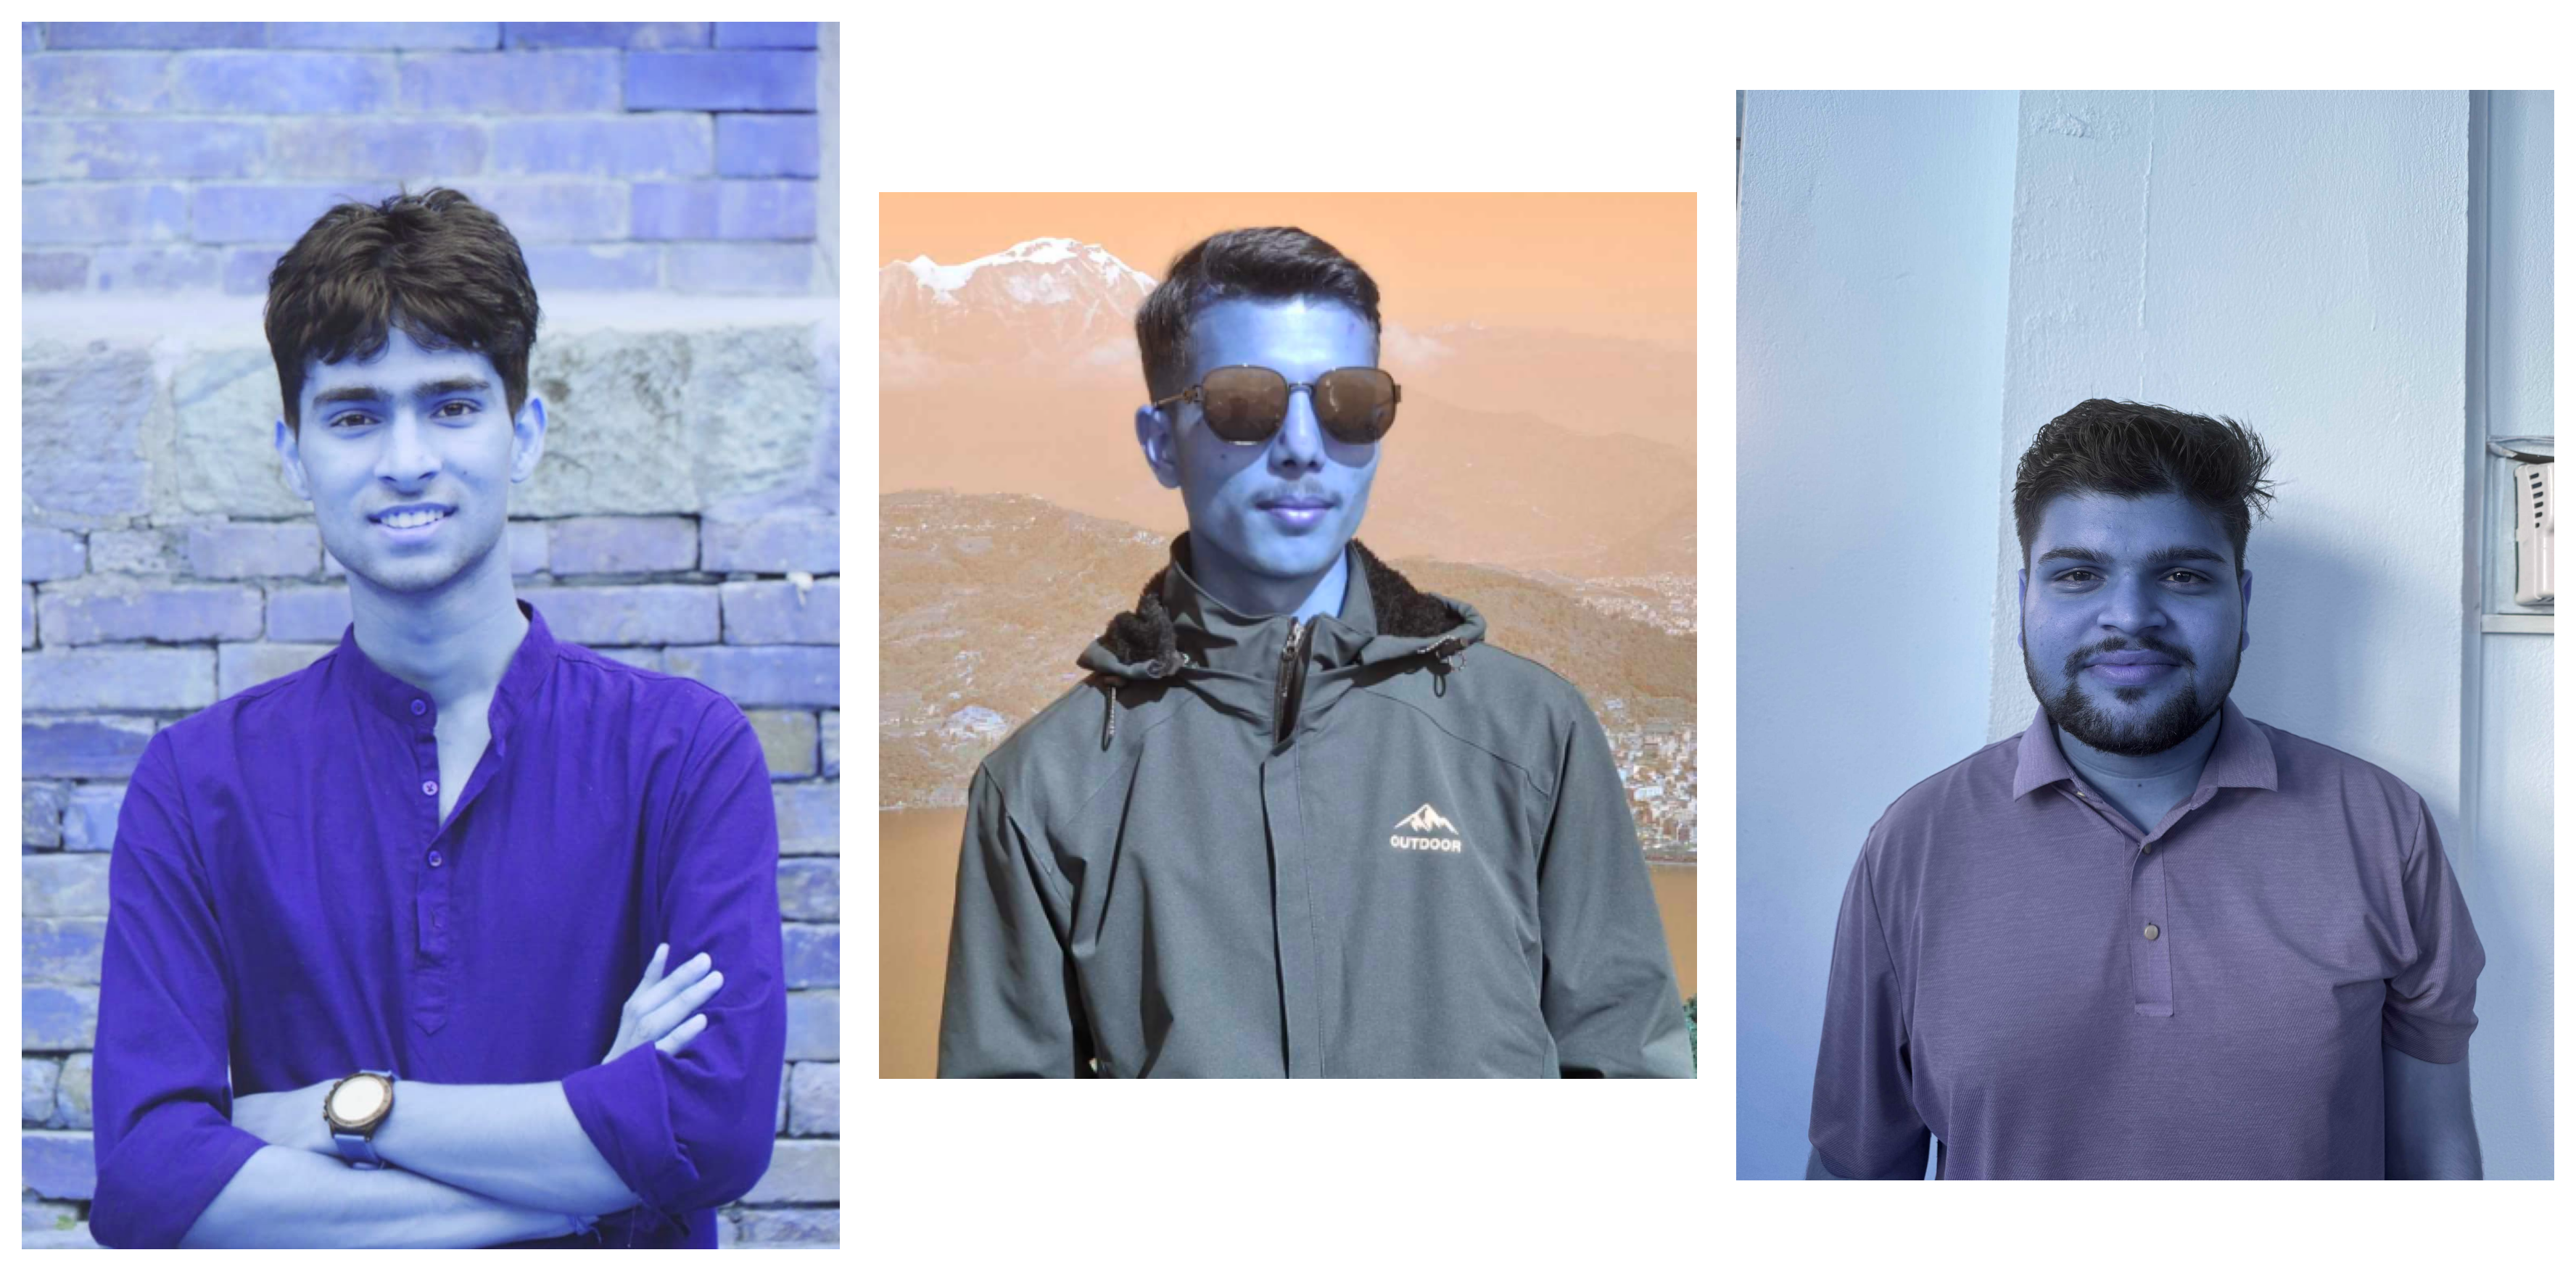
\includegraphics[width=\linewidth]{images/lab1/three_images_bgr.png}
  \caption{BGR representation of the test images}
  \label{fig:gray_images}
\end{figure}

We first loaded three test images and examined their properties:

\begin{lstlisting}[caption=Loading and displaying images]
import cv2
import matplotlib.pyplot as plt
import numpy as np

# Load images
img_1 = cv2.imread("bipul.jpeg")
img_2 = cv2.imread("bibek.png")
img_3 = cv2.imread("krishna.jpeg")

# Display images in RGB format
fig, axes = plt.subplots(1, 3, figsize=(12, 4))
axes[0].imshow(cv2.cvtColor(img_1, cv2.COLOR_BGR2RGB))
axes[1].imshow(cv2.cvtColor(img_2, cv2.COLOR_BGR2RGB))
axes[2].imshow(cv2.cvtColor(img_3, cv2.COLOR_BGR2RGB))
\end{lstlisting}

\subsubsection{Color Channel Separation}
To understand the contribution of each color channel to the overall image, we separated the RGB channels of our test images. For an RGB image, the channels can be accessed as:

\begin{lstlisting}[caption=Extracting RGB channels]
def return_rgb(image):
    r = image[:, :, 0]  # Red channel
    g = image[:, :, 1]  # Green channel
    b = image[:, :, 2]  # Blue channel
    return r, g, b
\end{lstlisting}

\begin{figure}[htbp]
  \centering
  \includegraphics[width=\linewidth]{images/lab1/three_images_rgb_channels.png}
  \caption{RGB channel separation of test images (top to bottom: first image, second image, third image; left to right: R, G, B channels)}
  \label{fig:channels}
\end{figure}

\subsubsection{Image Histograms}
A histogram represents the frequency distribution of pixel intensities in an image. It provides valuable information about contrast, brightness, and intensity distribution. For a digital image with intensity levels in the range $[0, L-1]$, the histogram is defined as:

\begin{equation}
  h(r_k) = n_k
\end{equation}

where $r_k$ is the $k^{th}$ intensity value and $n_k$ is the number of pixels with intensity $r_k$.

\begin{lstlisting}[caption=Creating image histograms]
def plot_histogram(image, title):
    r_ch = image[:, :, 0]
    g_ch = image[:, :, 1]
    b_ch = image[:, :, 2]

    plt.figure(figsize=(10, 5))
    plt.subplot(1, 3, 1)
    plt.hist(r_ch.ravel(), bins=256, color='red')
    plt.title(f'{title} - Red Channel Histogram')
    plt.subplot(1, 3, 2)
    plt.hist(g_ch.ravel(), bins=256, color='green')
    plt.title(f'{title} - Green Channel Histogram')
    plt.subplot(1, 3, 3)
    plt.hist(b_ch.ravel(), bins=256, color='blue')
    plt.title(f'{title} - Blue Channel Histogram')
\end{lstlisting}

\begin{figure}[htbp]
  \centering
  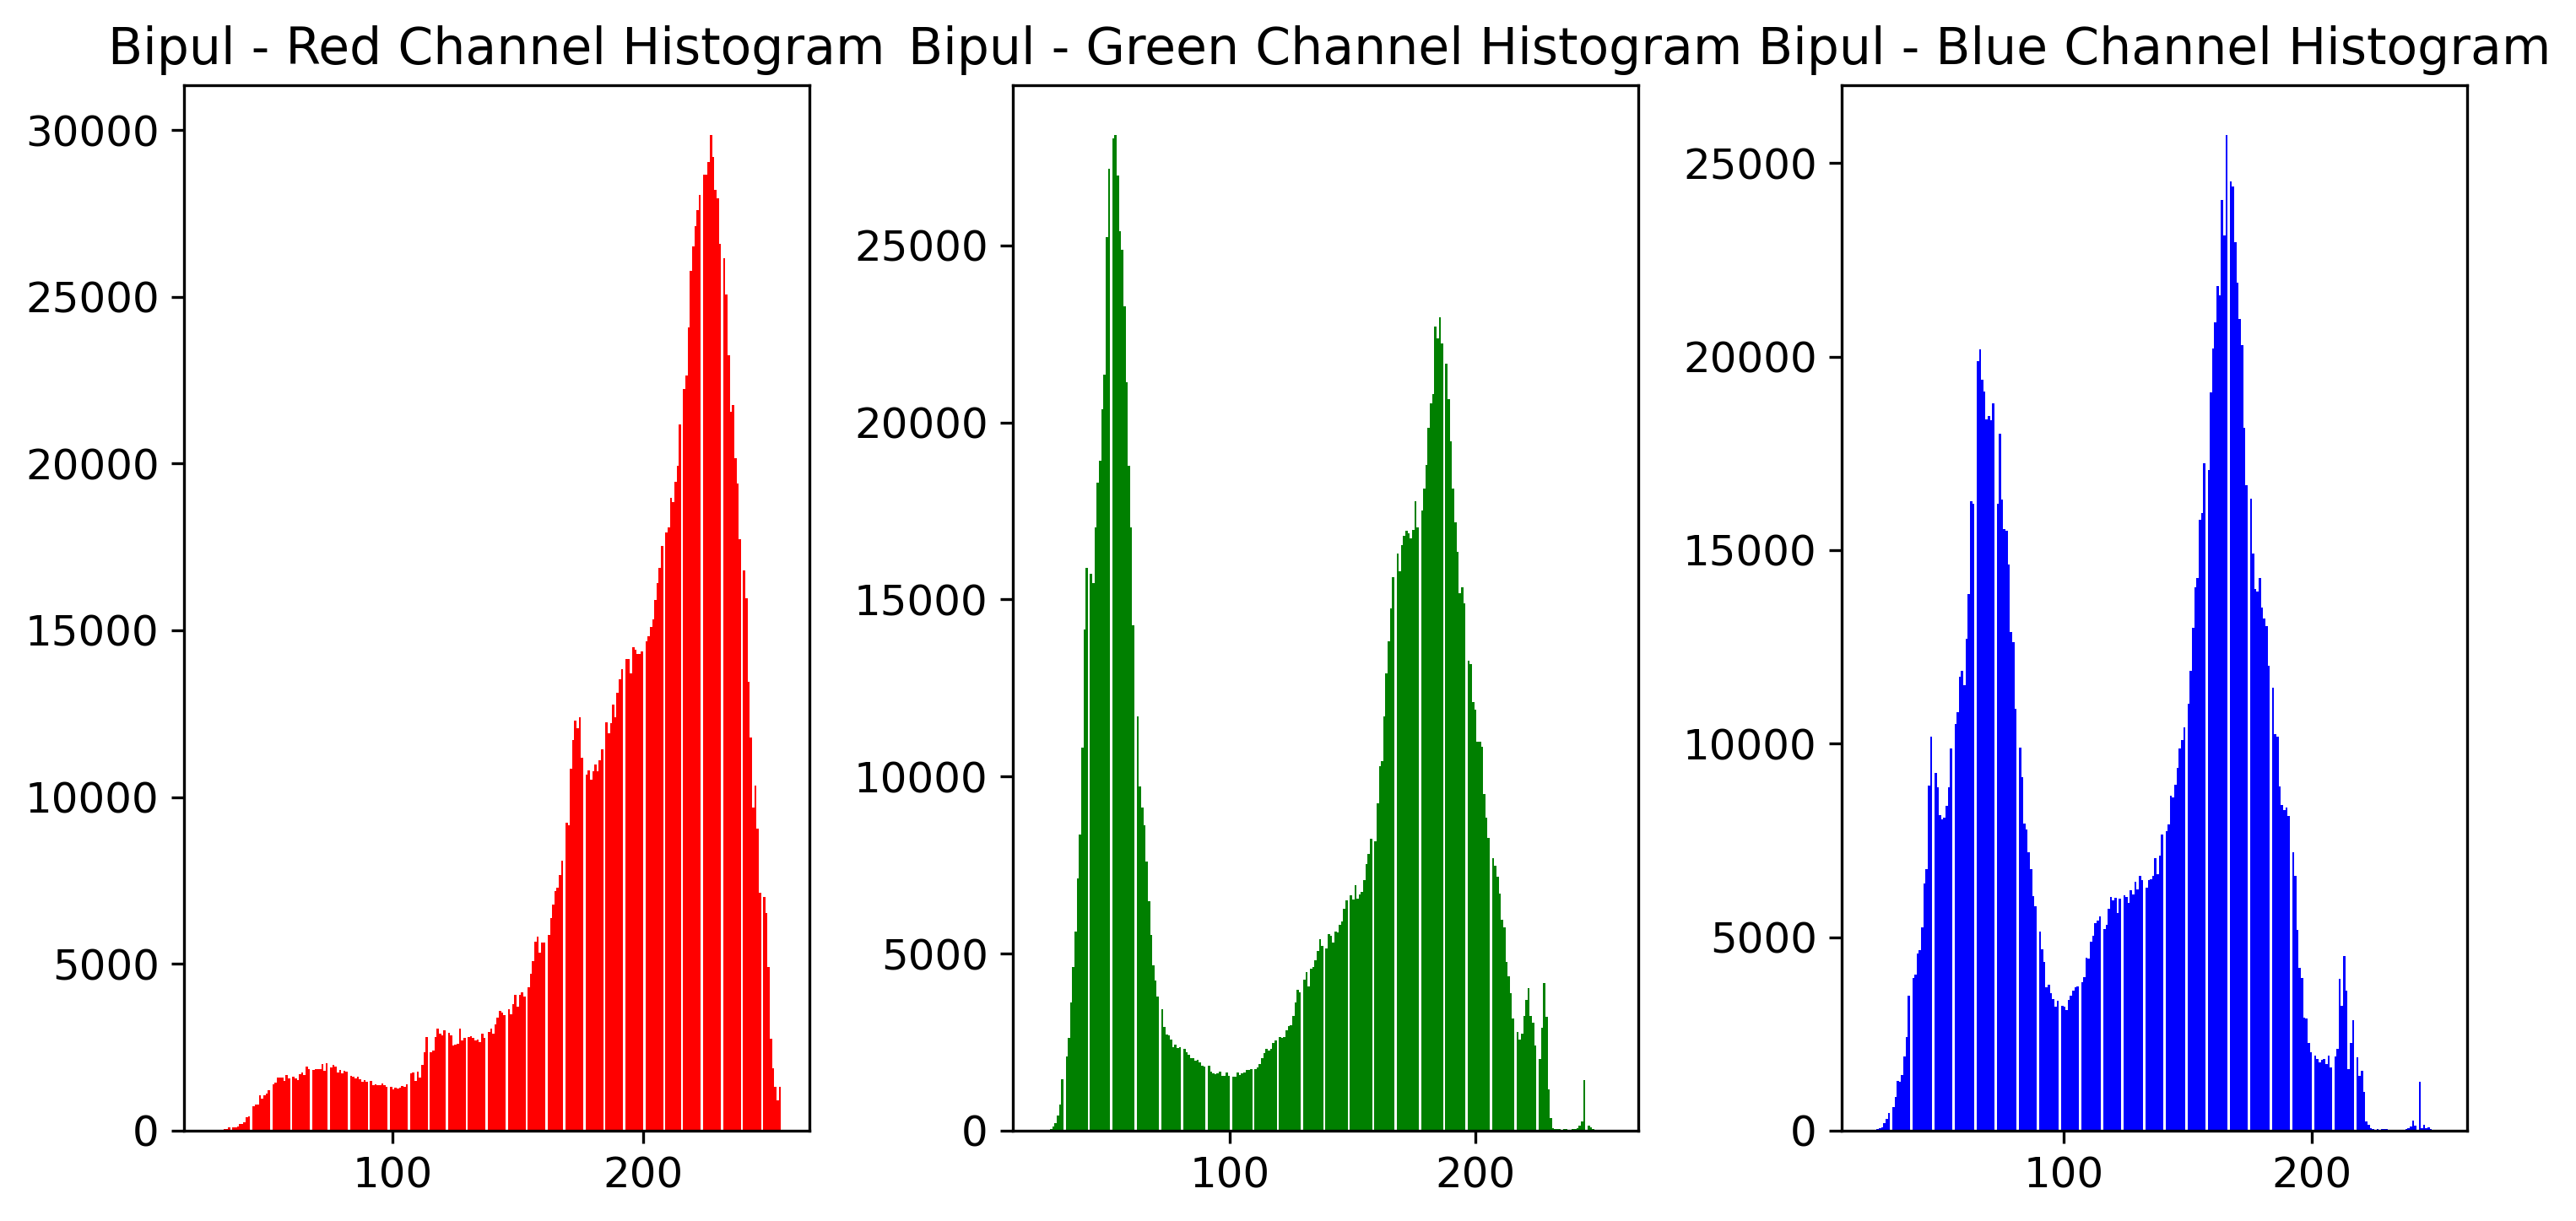
\includegraphics[width=\linewidth]{images/lab1/bipul_histogram.png}
  \caption{RGB channel histograms of the first test image}
  \label{fig:histogram1}
\end{figure}

\subsection{Image Enhancement}
Image enhancement techniques aim to improve the visual appearance of an image or to convert the image to a form better suited for analysis. We implemented several enhancement techniques in this experiment.


\subsubsection{Convolution Operation}
Convolution is a fundamental operation in image processing. The discrete convolution of an image $f$ with a kernel $h$ is given by:

\begin{equation}
  (f * h)(x, y) = \sum_{i=-a}^{a}\sum_{j=-b}^{b} f(x-i, y-j) \cdot h(i, j)
\end{equation}

where $h$ is a $(2a+1) \times (2b+1)$ convolution kernel. Our implementation:

\begin{lstlisting}[caption=2D convolution function]
def convolve2d(image, kernel):
    image_height, image_width = image.shape
    kernel_height, kernel_width = kernel.shape
    pad_height = kernel_height // 2
    pad_width = kernel_width // 2

    output_image = np.zeros((image_height, image_width))
    padded_image = np.pad(image, ((pad_height, pad_height), 
                                 (pad_width, pad_width)), 
                         mode='constant', constant_values=0)

    for i in range(image_height):
        for j in range(image_width):
            patch = padded_image[i:i + kernel_height, j:j + kernel_width]
            output_image[i, j] = np.sum(patch * kernel)
    return output_image
\end{lstlisting}

\subsubsection{Gaussian Filtering}
The Gaussian filter is widely used for image smoothing and noise reduction. The 2D Gaussian function is defined as:

\begin{equation}
  G(x, y) = \frac{1}{2\pi\sigma^2}e^{-\frac{x^2+y^2}{2\sigma^2}}
\end{equation}

where $\sigma$ is the standard deviation of the Gaussian distribution. In our implementation, we used a 3×3 Gaussian kernel:

\begin{equation}
  \frac{1}{16}
  \begin{bmatrix}
    1 & 2 & 1  \\
    2 & 4 & 2  \\
    1 & 2 & 1
  \end{bmatrix}
\end{equation}

\begin{lstlisting}[caption=Implementing a Gaussian filter]
gaussian_kernel = np.array([[1, 2, 1],
                           [2, 4, 2],
                           [1, 2, 1]]) / 16.0  # Normalized Gaussian kernel

def gaussian_filter(image):
    gray_image = cv2.cvtColor(image, cv2.COLOR_BGR2GRAY)
    gaussian_result = convolve2d(gray_image, gaussian_kernel)
    gaussian_result = np.clip(gaussian_result, 0, 255).astype(np.uint8)
    return gaussian_result
\end{lstlisting}


\begin{figure}[htbp]
  \centering
  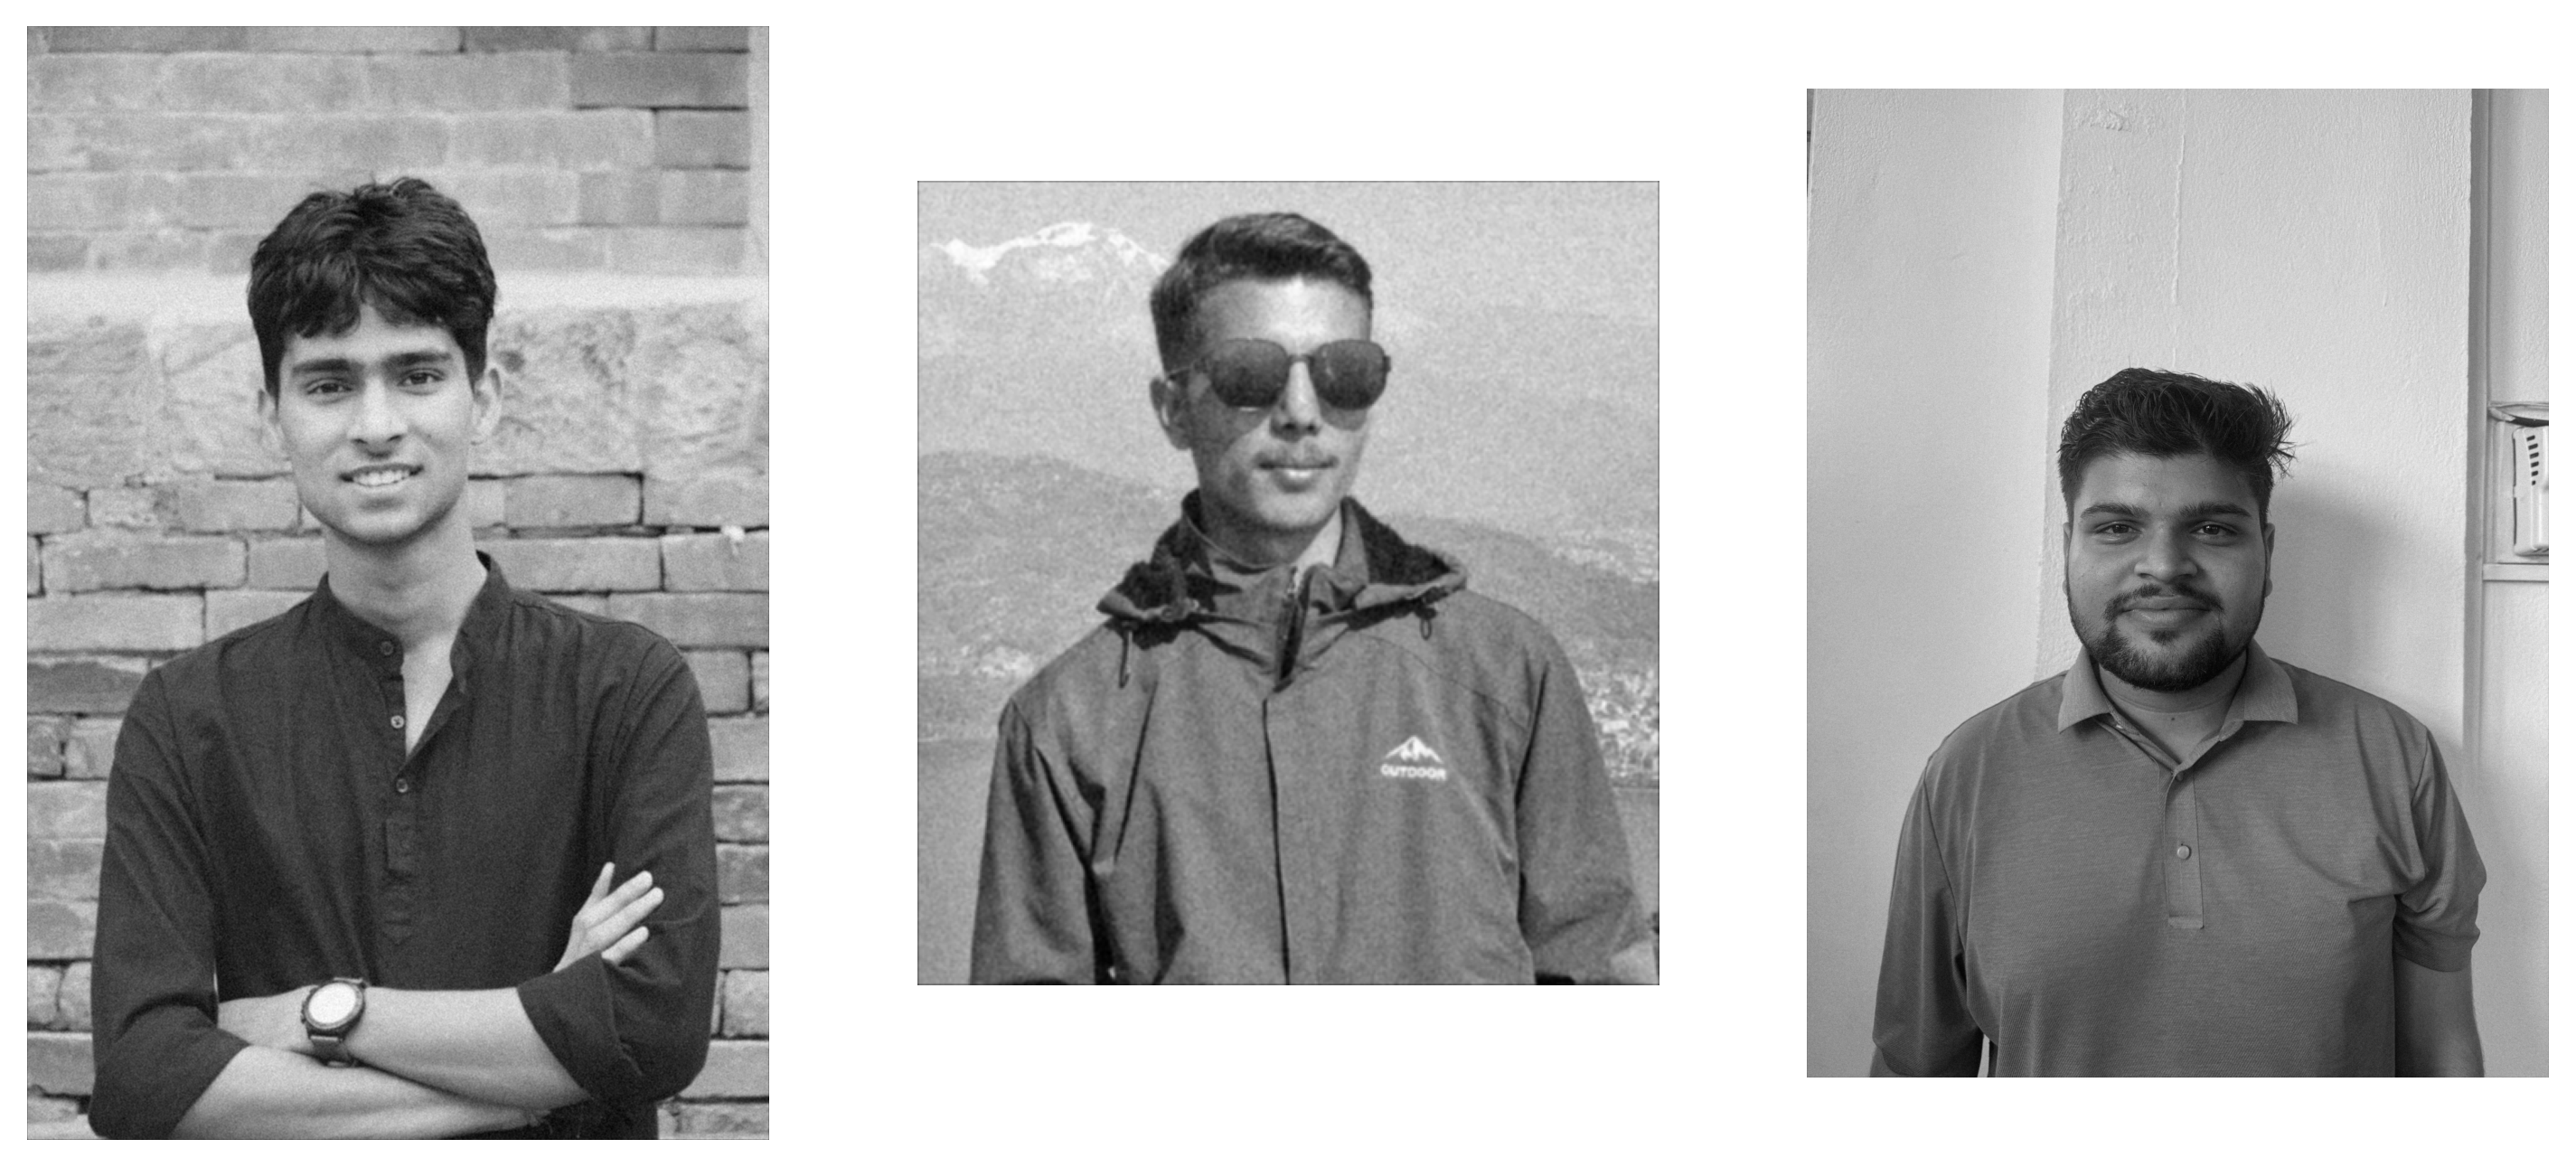
\includegraphics[width=\linewidth]{images/lab1/gaussian_filtered_images.png}
  \caption{Results of applying Gaussian filtering to noisy images}
  \label{fig:gaussian_filter}
\end{figure}

\subsection{Edge Detection}
Edge detection is a fundamental image processing technique used to identify boundaries within an image. Edges occur where there is a significant change in image intensity, indicating the boundaries of objects.

\subsubsection{Sobel Edge Detection}
The Sobel operator performs a 2-D spatial gradient measurement on an image to emphasize regions of high spatial frequency that correspond to edges. It consists of two 3×3 convolution kernels:

\begin{equation}
  G_x = 
  \begin{bmatrix}
    -1 & 0 & 1  \\
    -2 & 0 & 2  \\
    -1 & 0 & 1
  \end{bmatrix}
  \quad
  G_y = 
  \begin{bmatrix}
    1  & 2  & 1   \\
    0  & 0  & 0   \\
    -1 & -2 & -1
  \end{bmatrix}
\end{equation}

These kernels are convolved with the original image to calculate approximations of the derivatives - one for horizontal changes, and one for vertical changes. The magnitude of the gradient is then calculated as:

\begin{equation}
  G = \sqrt{G_x^2 + G_y^2}
\end{equation}

\begin{lstlisting}[caption=Implementing Sobel edge detection]
x_sobel = np.array([[-1, 0, 1],
                   [-2, 0, 2],
                   [-1, 0, 1]])

y_sobel = np.array([[1, 2, 1],
                   [0, 0, 0],
                   [-1, -2, -1]])

def sobel_filter(image):
    gray_image = cv2.cvtColor(image, cv2.COLOR_BGR2GRAY)
    sobel_x = convolve2d(gray_image, x_sobel)
    sobel_y = convolve2d(gray_image, y_sobel)

    sobel_magnitude = np.sqrt(sobel_x**2 + sobel_y**2)
    sobel_magnitude = np.clip(sobel_magnitude, 0, 255).astype(np.uint8)

    return sobel_magnitude
\end{lstlisting}

\begin{figure}[htbp]
  \centering
  \includegraphics[width=\linewidth]{images/lab1/sobel_filtered_images.png}
  \caption{Results of applying Sobel edge detection to test images}
  \label{fig:sobel_edge}
\end{figure}

\subsubsection{Laplacian Edge Detection}
The Laplacian operator is a second-order derivative operator that computes the second derivatives of an image, highlighting regions of rapid intensity change. The Laplacian of an image with pixel intensity values $I(x,y)$ is given by:

\begin{equation}
  \nabla^2I = \frac{\partial^2 I}{\partial x^2} + \frac{\partial^2 I}{\partial y^2}
\end{equation}

A common discrete approximation of the Laplacian function is:

\begin{equation}
  \nabla^2I = 
  \begin{bmatrix}
    0 & 1  & 0  \\
    1 & -4 & 1  \\
    0 & 1  & 0
  \end{bmatrix}
\end{equation}

\begin{lstlisting}[caption=Implementing Laplacian edge detection]
laplacian_kernel = np.array([[0, 1, 0],
                            [1, -4, 1],
                            [0, 1, 0]])

def laplacian_filter(image):
    gray_image = cv2.cvtColor(image, cv2.COLOR_BGR2GRAY)
    laplacian_result = convolve2d(gray_image, laplacian_kernel)
    laplacian_result = np.clip(laplacian_result, 0, 255).astype(np.uint8)
    return laplacian_result
\end{lstlisting}

\begin{figure}[htbp]
  \centering
  \includegraphics[width=\linewidth]{images/lab1/laplacian_filtered_images.png}
  \caption{Results of applying Laplacian edge detection to test images}
  \label{fig:laplacian_edge}
\end{figure}

\subsection{Image Segmentation}
Image segmentation is the process of partitioning an image into multiple segments to simplify or change the representation of an image into something more meaningful and easier to analyze. We implemented basic thresholding approaches for segmentation in this experiment.

\subsubsection{Thresholding}
Thresholding is the simplest method of image segmentation. From a grayscale image, thresholding can be used to create binary images. The basic thresholding operation can be defined as:

\begin{equation}
  g(x,y) = 
  \begin{cases}
    1, & \text{if } f(x,y) > T \\
    0, & \text{otherwise}
  \end{cases}
\end{equation}

where $T$ is the threshold value, $f(x,y)$ is the input image, and $g(x,y)$ is the resulting binary image.

\begin{lstlisting}[caption=Simple thresholding example]
def simple_threshold(image, threshold):
    gray = cv2.cvtColor(image, cv2.COLOR_BGR2GRAY)
    binary = gray > threshold
    return binary
\end{lstlisting}

\subsection{Noise Modeling and Restoration}
Image noise is random variation of brightness or color information in images. Noise modeling involves adding synthetic noise to images for testing denoising algorithms, while restoration aims to recover the original image from a noisy one.

\subsubsection{Gaussian Noise}
Gaussian noise is statistical noise with a probability density function equal to that of the normal distribution. It can be added to an image using:

\begin{equation}
  g(x,y) = f(x,y) + \eta(x,y)
\end{equation}

where $f(x,y)$ is the original image, $\eta(x,y)$ is the noise with normal distribution, and $g(x,y)$ is the resulting noisy image.

\begin{lstlisting}[caption=Adding Gaussian noise]
def add_noise_gaussian(image, noise_factor=0.1):
    noise = np.random.normal(loc=0, scale=noise_factor, size=image.shape)
    noisy_image = image + noise
    noisy_image = np.clip(noisy_image, 0, 255).astype(np.uint8)
    return noisy_image
\end{lstlisting}

\begin{figure}[htbp]
  \centering
  \includegraphics[width=\linewidth]{images/lab1/gaussian_noisy_images.png}
  \caption{Test images with added Gaussian noise}
  \label{fig:gaussian_noise}
\end{figure}

\subsubsection{Salt and Pepper Noise}
Salt and pepper noise refers to randomly occurring white and black pixels. It can be modeled as:

\begin{equation}
  g(x,y) = 
  \begin{cases}
    0,      & \text{with probability } p_p        \\
    255,    & \text{with probability } p_s        \\
    f(x,y), & \text{with probability } 1-p_p-p_s
  \end{cases}
\end{equation}

where $p_p$ is the probability of a pepper (black) noise and $p_s$ is the probability of a salt (white) noise.

\begin{lstlisting}[caption=Adding salt and pepper noise]
def add_salt_and_pepper_noise(image, salt_prob=0.02, pepper_prob=0.02):
    noisy_image = np.copy(image)
    total_pixels = image.size
    num_salt = np.ceil(salt_prob * total_pixels)
    num_pepper = np.ceil(pepper_prob * total_pixels)

    # Salt noise
    coords = [np.random.randint(0, i, int(num_salt)) for i in image.shape]
    noisy_image[coords[0], coords[1], :] = 255

    # Pepper noise
    coords = [np.random.randint(0, i, int(num_pepper)) for i in image.shape]
    noisy_image[coords[0], coords[1], :] = 0

    return noisy_image
\end{lstlisting}

\begin{figure}[htbp]
  \centering
  \includegraphics[width=\linewidth]{images/lab1/salt_and_pepper_images.png}
  \caption{Test images with added salt and pepper noise}
  \label{fig:sp_noise}
\end{figure}

\subsubsection{Image Restoration Techniques}

\paragraph{Gaussian Filter for Noise Removal}
We implemented a Gaussian filter for removing Gaussian noise:

\begin{lstlisting}[caption=Gaussian noise removal]
def restore_gaussian(image, kernel_size=5, sigma=1.0):
    kernel = cv2.getGaussianKernel(kernel_size, sigma)
    gaussian_kernel = np.outer(kernel, kernel)
    restored_image = cv2.filter2D(image, -1, gaussian_kernel)
    return restored_image
\end{lstlisting}

\begin{figure}[htbp]
  \centering
  \includegraphics[width=\linewidth]{images/lab1/restored_gaussian_images.png}
  \caption{Restored images after applying Gaussian filter to noisy images}
  \label{fig:gaussian_restoration}
\end{figure}

\paragraph{Median Filter for Salt and Pepper Noise}
The median filter is particularly effective at removing salt and pepper noise while preserving edges:

\begin{lstlisting}[caption=Salt and pepper noise removal using median filter]
def remove_salt_and_pepper(image, kernel_size=3):
    return cv2.medianBlur(image, kernel_size)
\end{lstlisting}

\begin{figure}[htbp]
  \centering
  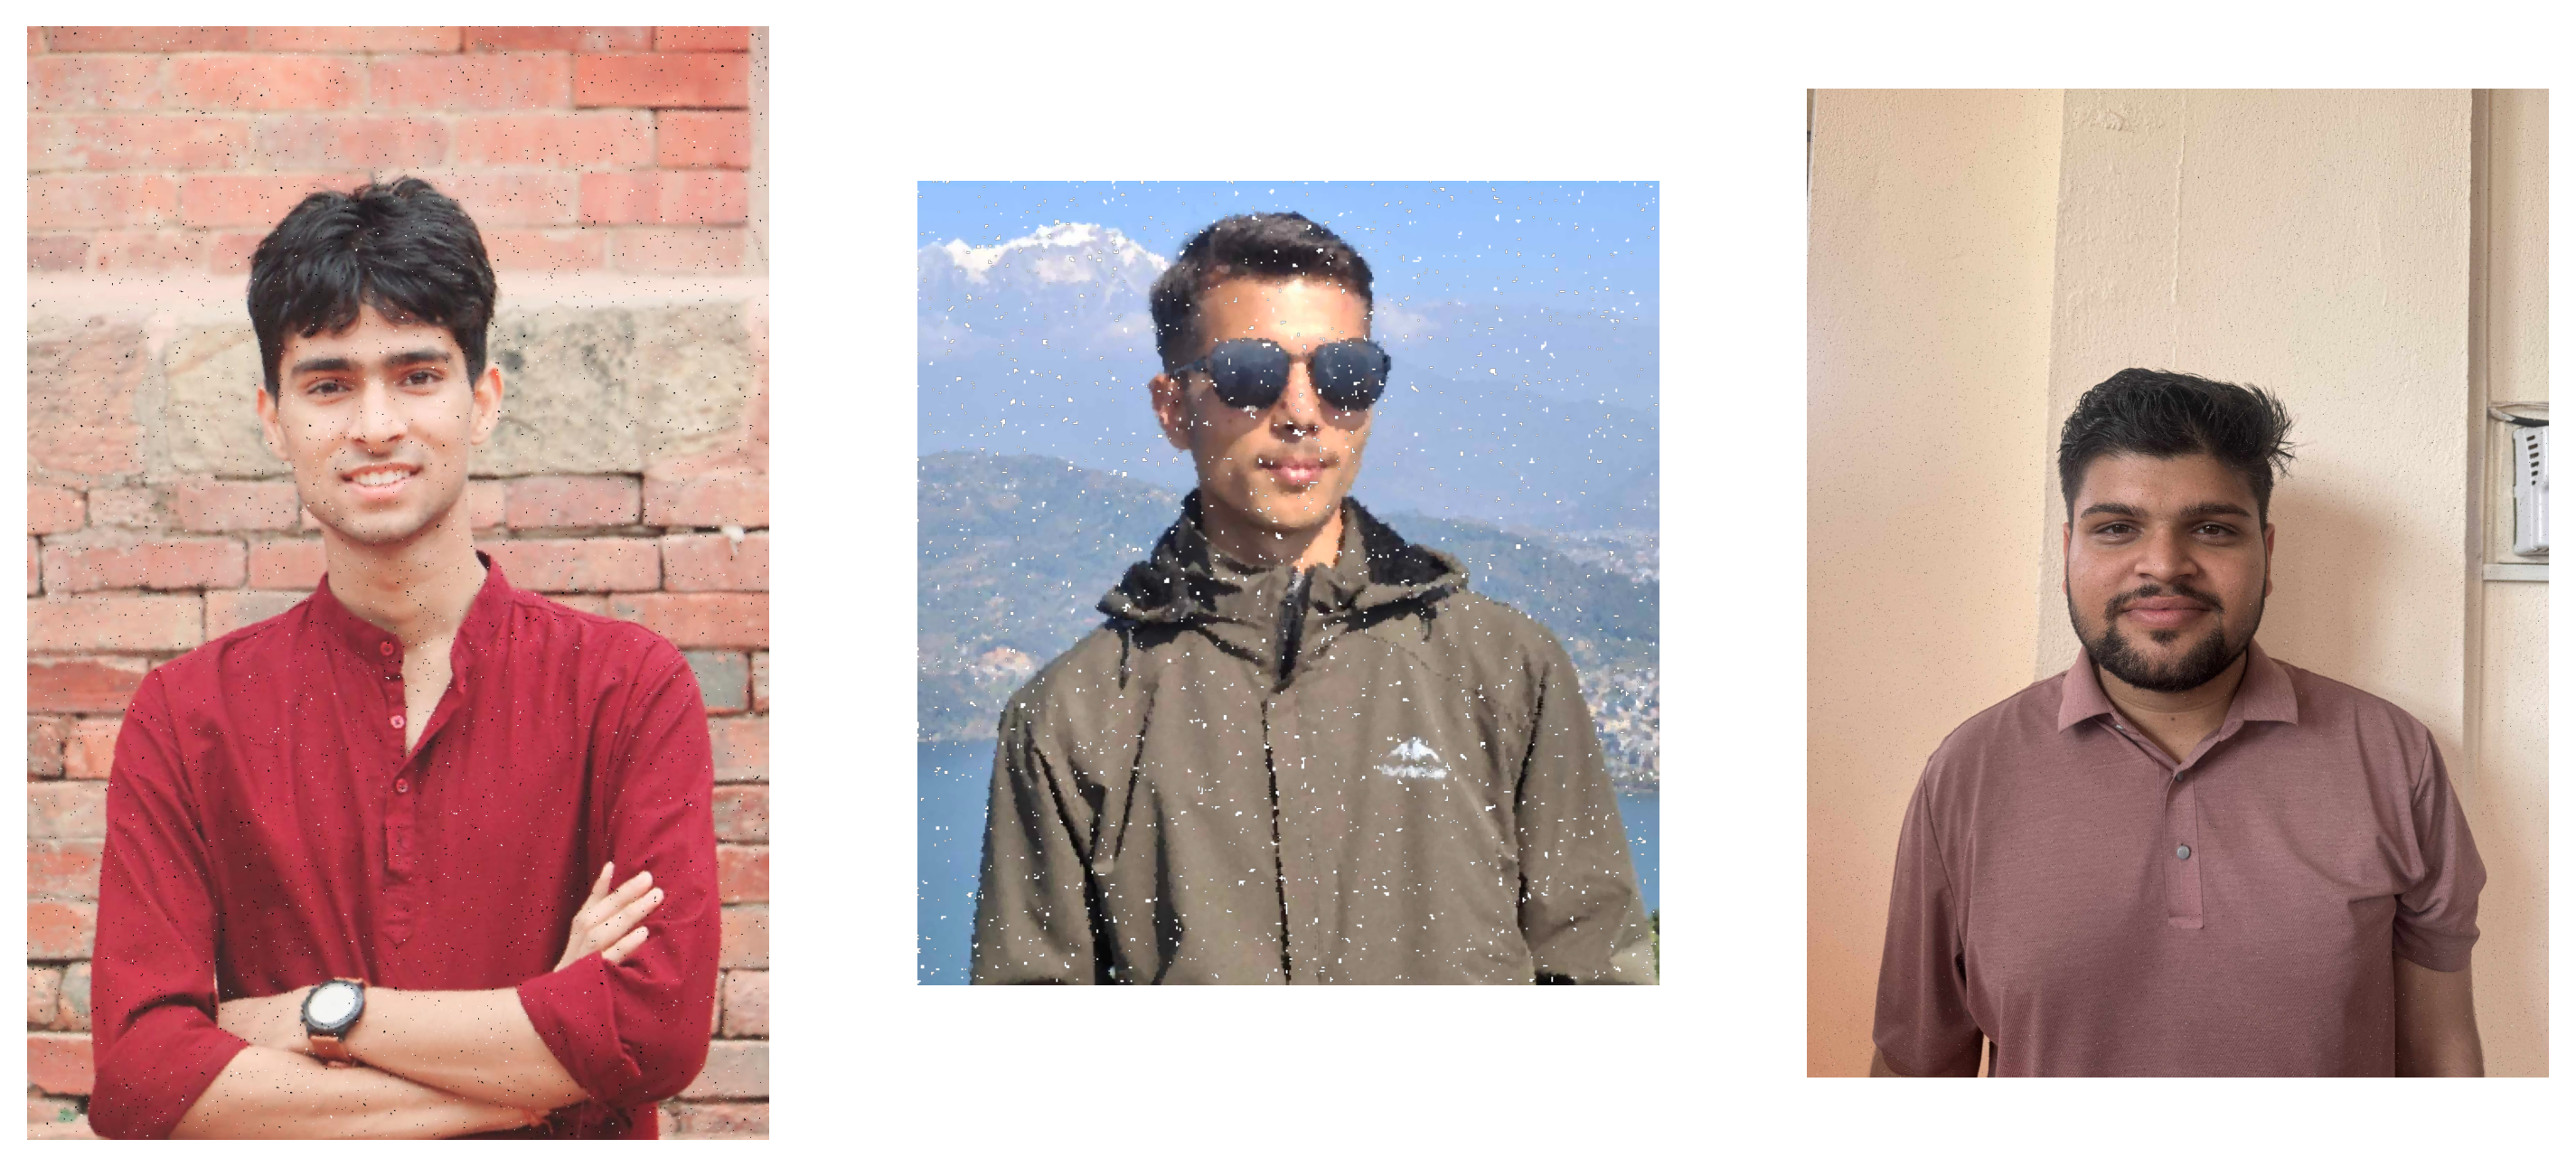
\includegraphics[width=\linewidth]{images/lab1/restored_salt_and_pepper_images.png}
  \caption{Restored images after applying median filter to noisy images}
  \label{fig:median_restoration}
\end{figure}


\section{Discussion}
The experimental results demonstrate the effectiveness of various image processing techniques:

\begin{itemize}
  \item \textbf{Edge Detection}: Both Sobel and Laplacian filters successfully highlighted image boundaries, with Sobel providing better directional edge information and Laplacian detecting finer edges.
        
  \item \textbf{Noise Modeling}: We successfully modeled two common types of image noise - Gaussian and salt-and-pepper - providing realistic test cases for restoration algorithms.
        
  \item \textbf{Image Restoration}: Gaussian filtering proved effective for removing Gaussian noise, while median filtering was particularly effective for salt-and-pepper noise removal.
        
  \item \textbf{Channel Separation}: By separating RGB channels, we observed that different channels capture different aspects of the image, with each channel's histogram revealing distinct intensity distributions.
\end{itemize}
These results highlight the importance of understanding image representation and processing techniques in practical applications, such as computer vision, medical imaging, and remote sensing.

\section{Conclusion}
This lab experiment provided practical experience with a range of image processing techniques using real photographs. We learned how to represent images as matrices, separate color channels, and analyze pixel intensity distributions with histograms. By applying filters like Sobel and Laplacian, we were able to detect edges and highlight important features in the images. We also explored how to add and remove different types of noise, using Gaussian filters for smoothing and median filters for cleaning up salt-and-pepper noise. These activities helped us understand how different methods work and when to use them. The skills gained from this lab are useful for many real-world tasks, such as improving image quality, finding objects in pictures, and preparing images for further analysis in areas like medical imaging and remote sensing.

\bibliographystyle{IEEEtran}
\bibliography{ref}

\end{document}